\pdfminorversion=4
\documentclass[xcolor={usenames,dvipsnames,svgnames,table}]{beamer}
%for printing or having a crappy pdf reader backup
%\documentclass[handout]{beamer}
\mode<presentation>
\usetheme{Madrid}

% this file contains all commonly used packages for the Rattlesnake documentation
% new package, add comment what they are used for

% command packages
\usepackage{xifthen}     % if -then else command

% language and font improvements
\usepackage[english]{babel}	% Multilingual support - https://www.ctan.org/pkg/babel
\usepackage[utf8]{inputenc} % Accept different input encodings - https://www.ctan.org/pkg/inputenc
\usepackage[kerning,spacing,babel]{microtype} % Subliminal refinements towards typographical perfection - https://www.ctan.org/pkg/microtype
\usepackage{eepic}      % Extensions to epic - https://www.ctan.org/pkg/eepic
\usepackage{epic}       % Enhance LaTeX picture mode - https://www.ctan.org/pkg/epic
\usepackage[T1]{fontenc} % selecting font encodingsselecting font encodings - https://www.ctan.org/pkg/fontenc
\usepackage{lmodern}

% title packages
\usepackage{authblk}		% footnote style author/affiliation - https://www.ctan.org/pkg/authblk

% symbols
\usepackage{upgreek}		% Upright Greek letters - https://www.ctan.org/pkg/upgreek
\usepackage{cancel}			% \cancel cmd - https://www.ctan.org/pkg/cancel

% chemical and isotope packages
\usepackage{isotope}		% isotope command - https://www.ctan.org/pkg/isotope
\usepackage{mhchem}			% chemical formulae/equations - https://www.ctan.org/pkg/mhchem

% layout packages
\usepackage{xspace}			% smart space \xspace - https://www.ctan.org/pkg/xspace
\usepackage{icomma}			% smart math comma - https://www.ctan.org/pkg/icomma
\usepackage{chngpage}		% page layout change during document - https://www.ctan.org/pkg/chngpage
\usepackage[usenames,dvipsnames,svgnames,table]{xcolor}			% color definitions - https://www.ctan.org/pkg/xcolor
\usepackage{enumitem}   % layout for itemize and enumerate - http://www.ctan.org/pkg/enumitem
\usepackage{setspace}    % allows for \singlespacing, \onehalfspacing, and \doublespacing commands - https://www.ctan.org/pkg/setspace

% floating packages
% needed by the breakalgo environment labelsep=quad
\usepackage[singlelinecheck=false, labelsep=quad]{caption}	% table captions - https://www.ctan.org/pkg/caption
\usepackage{subcaption}		% Support for sub-captions - https://www.ctan.org/pkg/subcaption
\usepackage{placeins}   	% Control float placement - https://www.ctan.org/pkg/placeins
\usepackage{float}      	% Improved interface for floating objects - https://www.ctan.org/pkg/float

% table packages
\usepackage{supertabular}	% multi-page tables package - https://www.ctan.org/pkg/supertabular
\usepackage{booktabs}		% table settings - https://www.ctan.org/pkg/booktabs
\usepackage{array}			% Extending the array and tabular environments - https://www.ctan.org/pkg/array
\usepackage{multirow}		% tabular cells spanning multiple rows - https://www.ctan.org/pkg/multirow
% \usepackage{tabls}      % Better vertical spacing in tables and arrays - https://www.ctan.org/pkg/tabls
\usepackage{colortbl}      % Allows for color manipulation within tables - https://www.ctan.org/pkg/colortbl

% pictures, plots and listings
\usepackage{graphicx}		% include graphics - https://www.ctan.org/pkg/graphicx
\usepackage{wrapfig}		% wrapfigure enviroment - https://www.ctan.org/pkg/wrapfig
\usepackage{pgfplots}		% latex plots - https://www.ctan.org/pkg/pgfplots


% source code and algorithms
\usepackage{algorithmicx} % newer version of algorithmic - https://www.ctan.org/pkg/algorithmicx
\usepackage{listings} 	% source code listings - http://www.ctan.org/pkg/listings
\usepackage{verbatim}   % verbatim - https://www.ctan.org/pkg/verbatim

% misc packages
\usepackage{url}        % provide \url command for web addresses - https://www.ctan.org/pkg/url
\usepackage{import}			% Establish input relative to a directory - https://www.ctan.org/pkg/import
\usepackage{afterpage}  % Execute command after the next page break - https://www.ctan.org/pkg/afterpage
\usepackage{lscape}     % Place selected parts of a document in landscape - https://www.ctan.org/pkg/lscape
\usepackage{rotating}   % Rotation tools, including rotated full-page floats - https://www.ctan.org/pkg/rotating
\usepackage{chngcntr}   % Change the resetting of counters - http://ctan.org/pkg/chngcntr
\usepackage{textpos}    % Allows logo and banner manipulation

% eps support
\usepackage{epsfig}       % include eps figures - https://www.ctan.org/pkg/epsfig
\usepackage{epsf}          % Simple macros for EPS inclusion - https://www.ctan.org/pkg/epsf
\usepackage{epstopdf}   %use .eps images (as pdf) in \includegraphics


% reference packages
% hyperref must be loaded before amsmath to avoid problems with subequations and align
\usepackage{hyperref}		% Extensive support for hypertext - https://www.ctan.org/pkg/hyperref


% packages that must be loaded after hyperref - http://tex.stackexchange.com/questions/1863/which-packages-should-be-loaded-after-hyperref-instead-of-before
\usepackage{geometry}		% Flexible and complete interface to document dimensions - https://www.ctan.org/pkg/geometry
\usepackage{algorithm}  % algorithm enviroment

% ams math packages
\usepackage{amsmath}    % mathematical facilities - https://www.ctan.org/pkg/amsmath
\usepackage{amsfonts}   % fonts for math - https://www.ctan.org/pkg/amsfonts
\usepackage{amssymb}    %
\usepackage{amsthm}     % Typesetting theorems - https://www.ctan.org/pkg/amsthm

\usepackage{nameref}		% allows references with names instread of numbers \nameref - http://www.ctan.org/pkg/nameref
\usepackage[capitalize,nameinlink]{cleveref}   % smart references - http://ctan.org/pkg/cleveref

\makeatletter
% prevent a package from loading
\newcommand{\dontusepackage}[2][]{%
    \@namedef{ver@#2.sty}{9999/12/31}%
    \@namedef{opt@#2.sty}{#1}
}

% a macro to load packages only if they are not yet loaded, needed for combination of beamer and hyperref
\newcommand{\usepackagesave}[2][{}]{
    \ltx@ifpackageloaded{#2}{}{
        \usepackage[#1]{#2}}
}
\makeatother
%Prevent authblk from loading
\dontusepackage{authblk}


\usecolortheme[RGB={128,128,128}]{structure}
\definecolor{my_gray}{RGB}{105,105,105}
\setbeamercolor{khumna}{fg=white,bg=my_gray}
%teal \usecolortheme[RGB={0,128,128}]{structure}
%\useoutertheme{miniframes}
\useinnertheme{default}
\definecolor{Maroon}{RGB}{80,0,0}
\definecolor{BurntOrange}{RGB}{204,85,0}

\usepackage[figurename=,tablename=]{caption}
\setbeamercolor{normal text}{fg=black}
\setbeamercovered{dynamic}
\beamertemplatetransparentcovereddynamicmedium
\setbeamertemplate{caption}[numbered]
\usepackage{colortbl}
\newcommand {\mathsym}[1]{{}}
\newcommand {\unicode}{{}}
\newcommand{\om}{\boldsymbol{\Omega}}
\newcommand{\etal}{{\it et al.\,}}
\newcommand{\vr}{\vec{r}}
\newcommand{\vo}{\vec{\Omega}}
\newcolumntype{L}{>{\centering\arraybackslash}m{3cm}}
\newcommand{\tcr}[1]{\textcolor{red}{#1}}
%Creating a norm command
\newcommand{\norm}[1]{\left\lVert#1\right\rVert}
%Allow page breaks within align
\allowdisplaybreaks



\newlength \figwidth
\setlength \figwidth {0.5\textwidth}

\newcommand{\backupbegin}{
   \newcounter{finalframe}
   \setcounter{finalframe}{\value{framenumber}}
}
\newcommand{\backupend}{
   \setcounter{framenumber}{\value{finalframe}}
}

\addtobeamertemplate{frametitle}{}
{
	\begin{textblock*}{100mm}(0.85\textwidth,-1cm)
	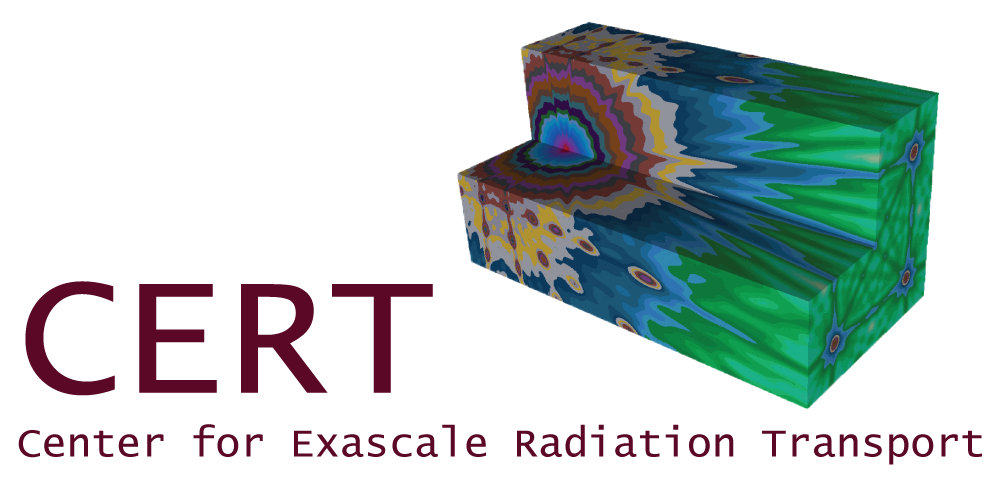
\includegraphics[height = 1cm,width=2cm]{figures/cert_logo_maroon.png}
	\end{textblock*}
}
\beamertemplatenavigationsymbolsempty



\begin{document}
%	

\title[Partitioning Optimization]{Partitioning Optimization for Massively Parallel Transport Sweeps on Unstructured Grids}
\author[Ghaddar]{Tarek Ghaddar}
\institute[TAMU]{Tarek Ghaddar \\ Texas A\&M University \\ ORNL Interview Seminar}
\date[May 14, 2018]

{
\setbeamertemplate{headline}{}
\begin{frame}
\vspace{-1.1cm}
	\begin{figure}[t]
		\centering
			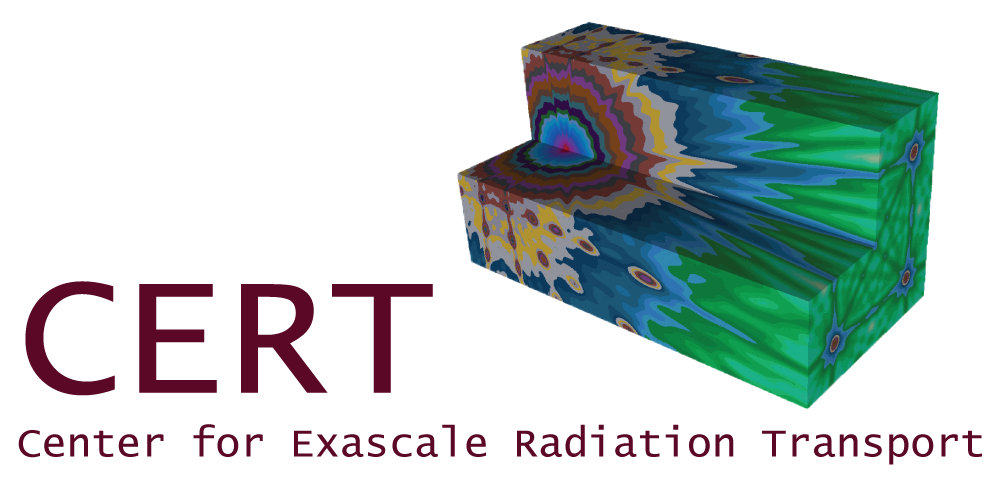
\includegraphics[width=.25\textwidth]{figures/cert_logo_maroon.png}
	\end{figure}
\vspace{-0.75cm}
\titlepage
\end{frame}
}

\setbeamertemplate{footline}
{

%\vspace{-0.1ex}
\begin{beamercolorbox}[wd=\textwidth,ht=3.5ex]{khumna}

\includegraphics[width = 0.95\textwidth]{figures/cert_banner.pdf}
	%\begin{textblock*}{10mm}(0.95\textwidth,10cm)
	\insertframenumber/\inserttotalframenumber
	%\end{textblock*}
\end{beamercolorbox}
%\begin{beamercolorbox}[wd=0.05\textwidth,ht=3.5ex]{khumna}

%\end{beamercolorbox}
}

\begin{frame}
\tableofcontents
\end{frame}

\section{Introduction and Background}

\begin{frame}[t]\frametitle{Introduction}
\begin{block}{}
\begin{itemize}
	\item Massively parallel transport sweeps have been shown to scale up to 750,000 cores on logically cartesian grids.
	\item Structured meshes are somewhat limiting when attempting to simulate more complex problems and experiments.
	\item Unstructured meshes allow us to simulate realistic problems, but introduce unbalanced partitions. 
	\item PDT (Texas A\&M's massively parallel transport code) introduced two load balancing algorithms that repartition the mesh in order to obtain a roughly equivalent amount of cells per processor. 
	\item However, this can sacrifice the optimal sweep partitioning (cut lines all the way through the domain) in favor of balance. 
	\item The method described will balance perfect load balancing and optimal sweep partitioning in order to achieve the best possible time to solution.
\end{itemize}
\end{block}
\end{frame}

\begin{frame}[t]\frametitle{Transport Sweeps}
\begin{block}{}
\begin{equation}
\vo_m \cdot \vec\nabla \psi_m^{(l+1)}(\vr) + \Sigma_t \psi_m^{(l+1)}(\vr) = q_m^{(l)}(\vr),
\label{iteration}
\end{equation}
\begin{itemize}
\item The domain is meshed and discretized, allowing one cell at a time to be solved.
\item The solution across a cell interface is connected based on an upwind approach.
\end{itemize}
\end{block}
\centering
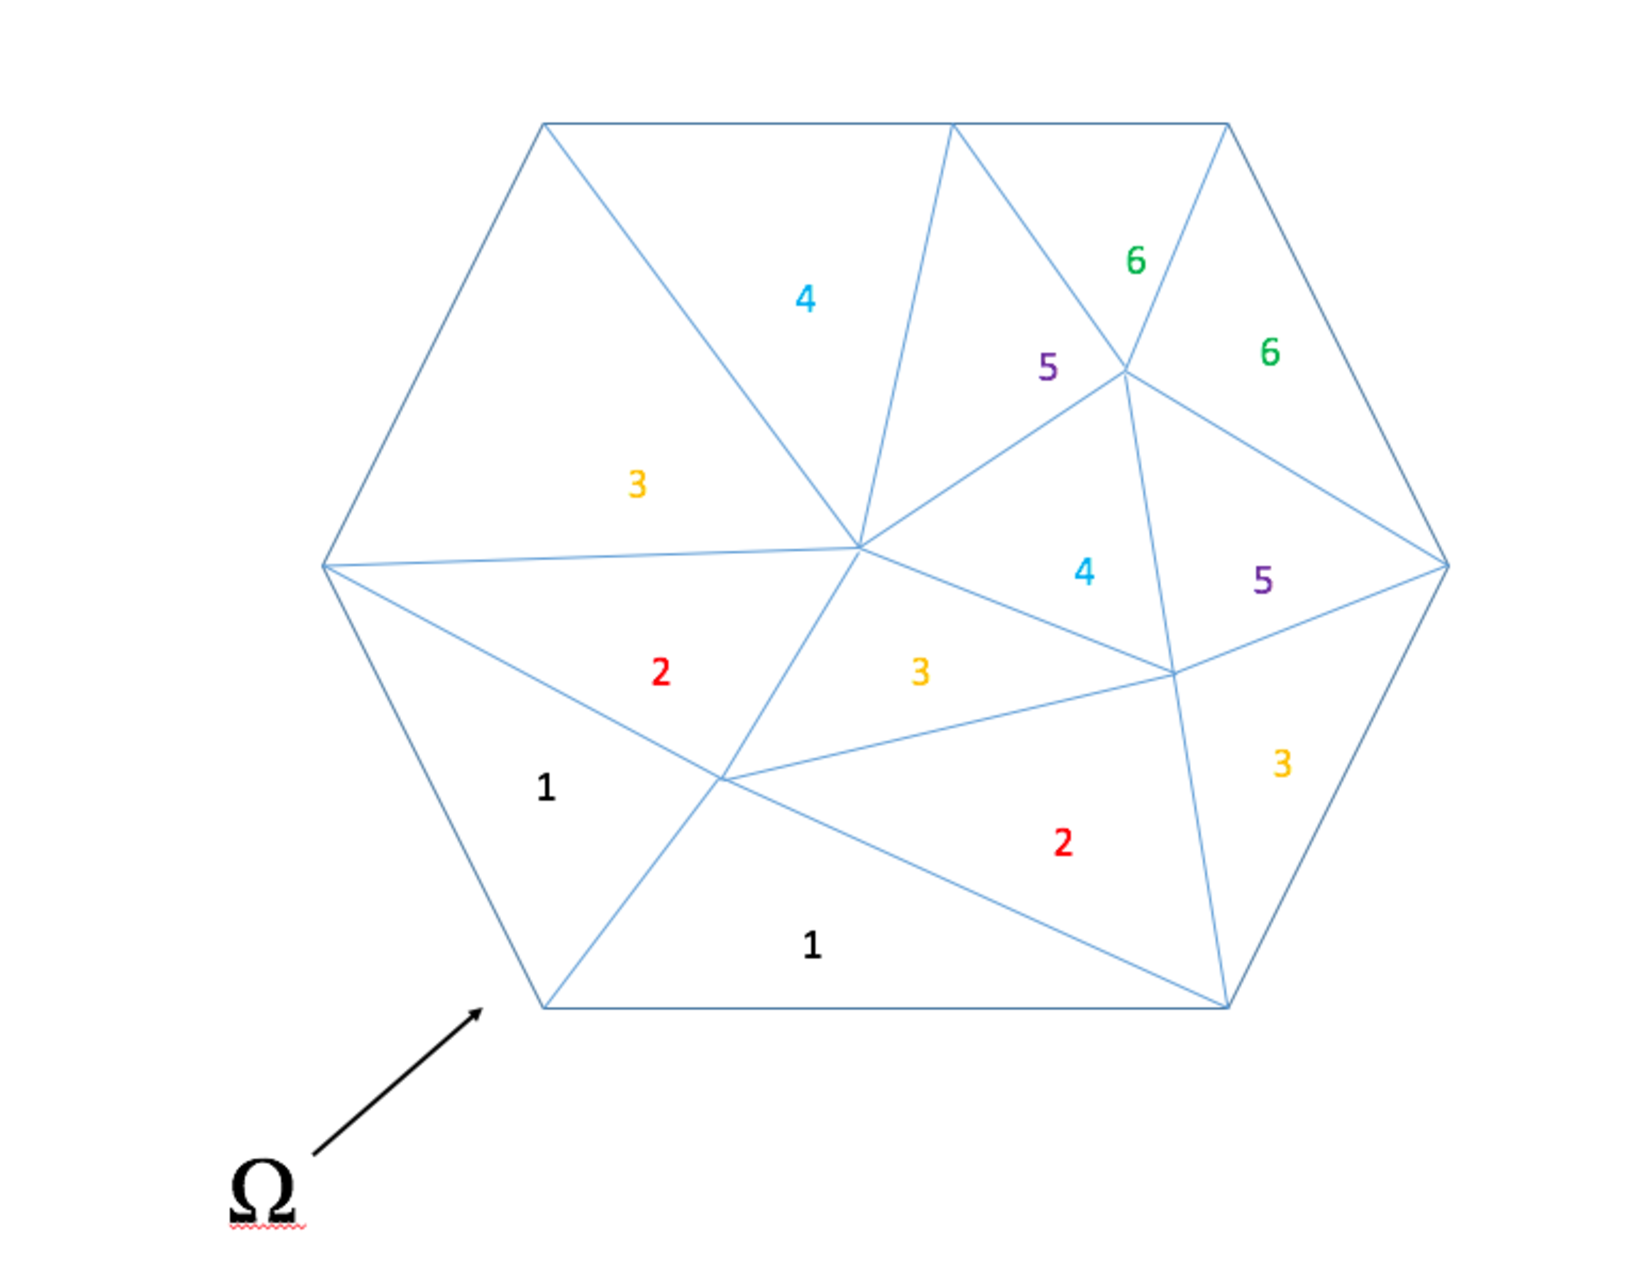
\includegraphics[scale = 0.15]{figures/UnstructureMesh.pdf}
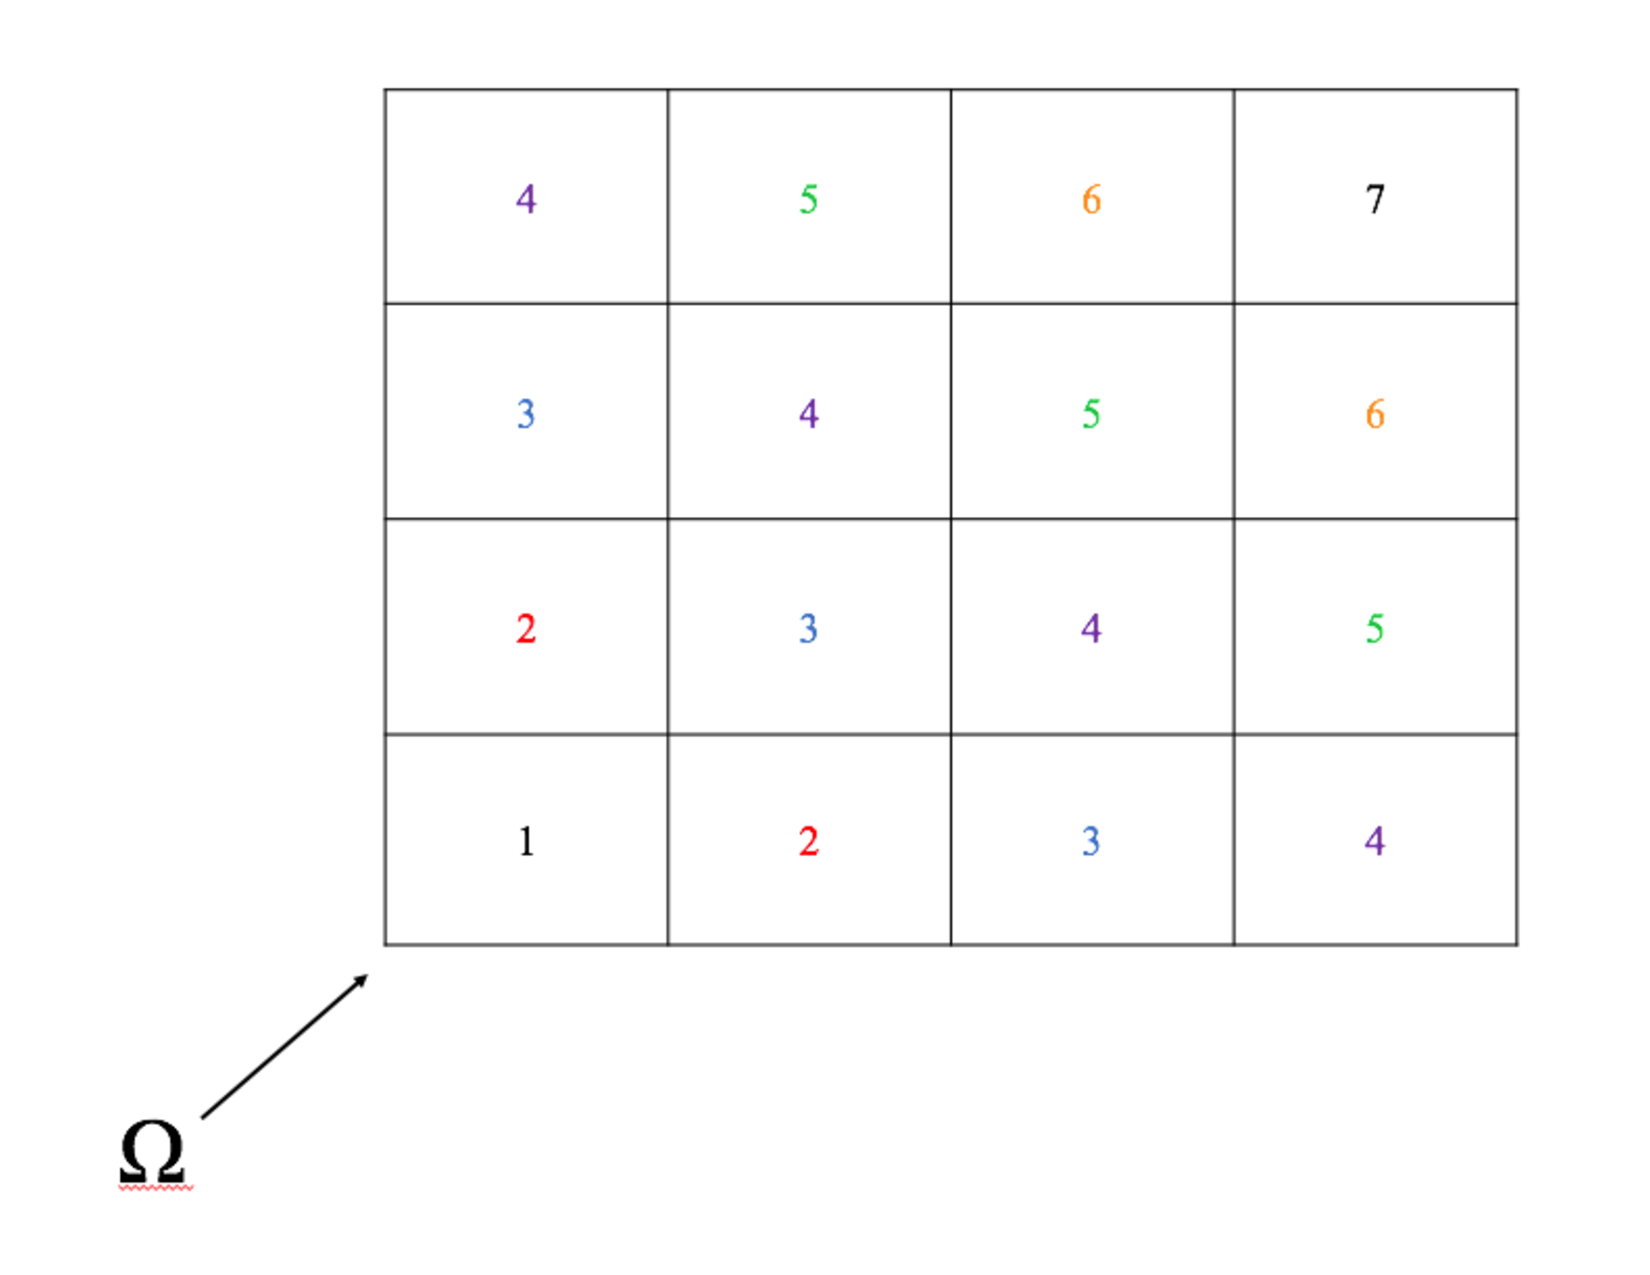
\includegraphics[scale = 0.15]{figures/StructuredMesh.pdf}
\end{frame}

\begin{frame}[t]\frametitle{Parallel Transport Sweeps}

\begin{block}{A parallel sweep algorithm is defined by three properties:}
\begin{itemize}
\item partitioning: dividing the domain among available processors,
\item aggregation: grouping cells, directions, and energy groups into tasks,
\item scheduling: choosing which task to execute if more than one is available.
\end{itemize}
\end{block}
\end{frame}


\begin{frame}[t]\frametitle{KBA Algorithm}
\begin{block}{}
\begin{itemize}
\item KBA limits the number of processors in $z$ to one, solves one group at a time, and does not aggregate in angle or group.
\item KBA primarily uses a "successive in angle, successive in quadrant" approach.
\item An octant pipelines its angular work, and once all directions are complete, the opposing octant pipelines them back.
\item This is then done for all remaining octant pairs.
\end{itemize}
\end{block}
\end{frame}

\begin{frame}[t]\frametitle{KBA Algorithm}
\begin{block}{}
\begin{itemize}
\item KBA utlilizes a "pipelining" or assembly line approach where new work is started before old work is fully completed.
\end{itemize}
\end{block}
\centering
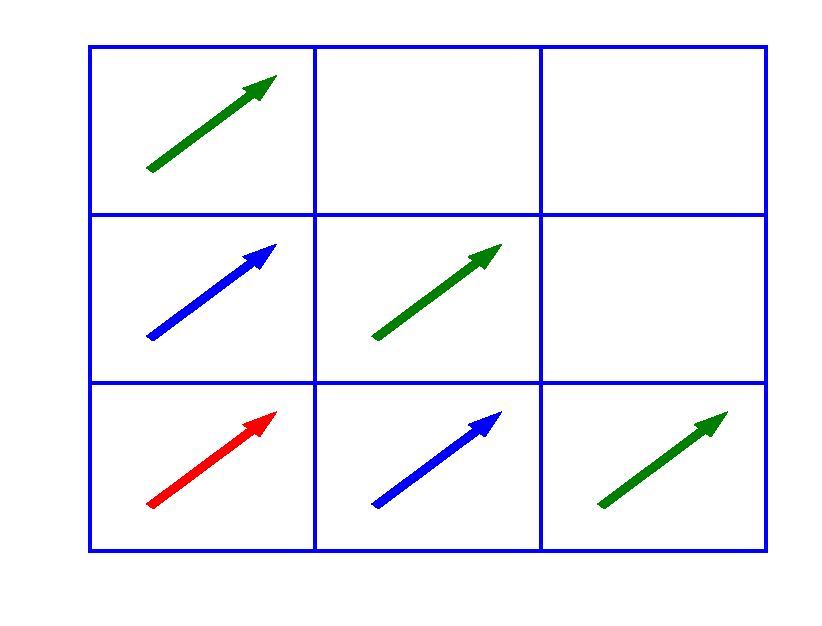
\includegraphics[scale=0.6,trim={0cm 1cm 0cm 0cm},clip]{../figures/pipeline_example.pdf}
\end{frame}

\begin{frame}[t]\frametitle{Sweeps in PDT}
\begin{block}{}
\begin{itemize}
\item PDT's extension of the KBA algorithm does not limit $P_z, A_m, G,$ or $A_g$.
\item PDT also launches all 8 octants (4 quadrants in 2D) simultaneously, rather than one octant-pair at a time.
\item Unlike KBA, PDT must schedule around conflicts that emerge between octants.
\end{itemize}
\end{block}
\end{frame}

\begin{frame}[t]\frametitle{Tie Breaking in PDT}

\begin{block}{If two or more tasks reach a processor at the same time, PDT employs a tie breaking strategy:}

\begin{enumerate}
	\item The task with the greater depth-of-graph remaining (simply, more work remaining) goes first.
	\item If the depth-of-graph remaining is tied, the task with $\Omega_x > 0$ wins.
	\item If multiple tasks have $\Omega_x > 0$, then the task with $\Omega_y > 0$ wins.
	\item If multiple tasks have $\Omega_y > 0$, then the task with $\Omega_z > 0$ wins.
\end{enumerate}
\end{block}
\end{frame}

\section{Unstructured Meshing}

\begin{frame}[t]\frametitle{Unstructured Meshing in PDT}
  \begin{block}{}
    \begin{itemize}
      \item PDT using unstructured meshes has been a priority since early 2014. 
      \item Unstructured meshes allow for simulation of a wider and more general variety of problems.
      \item Two unstructured mesh types are supported in PDT:
        \begin{itemize}
          \item Triangle (2D and 2D extruded triangular/prismatic meshes).
          \item Cubit/OpenFOAM (fully unstructured 2D/3D meshes).
        \end{itemize}
    \end{itemize}
  \end{block}
\end{frame}

\begin{frame}[t]\frametitle{Unstructured Meshing in PDT}
\begin{block}{Partitioning for Unstructured Meshes}
\begin{itemize}
\item ``Cut lines" in 2D (cut planes for 3D) are used to slice through the mesh in the $x$, $y$, and $z$ dimensions.
\item The cut planes form brick partitions, called subsets, that have unstructured meshes inside of them. 
\item The subsets are distributed amongst the processor domain.
\end{itemize}
\end{block}
\end{frame}

\begin{frame}[t]\frametitle{Partitioning Example}
\centering
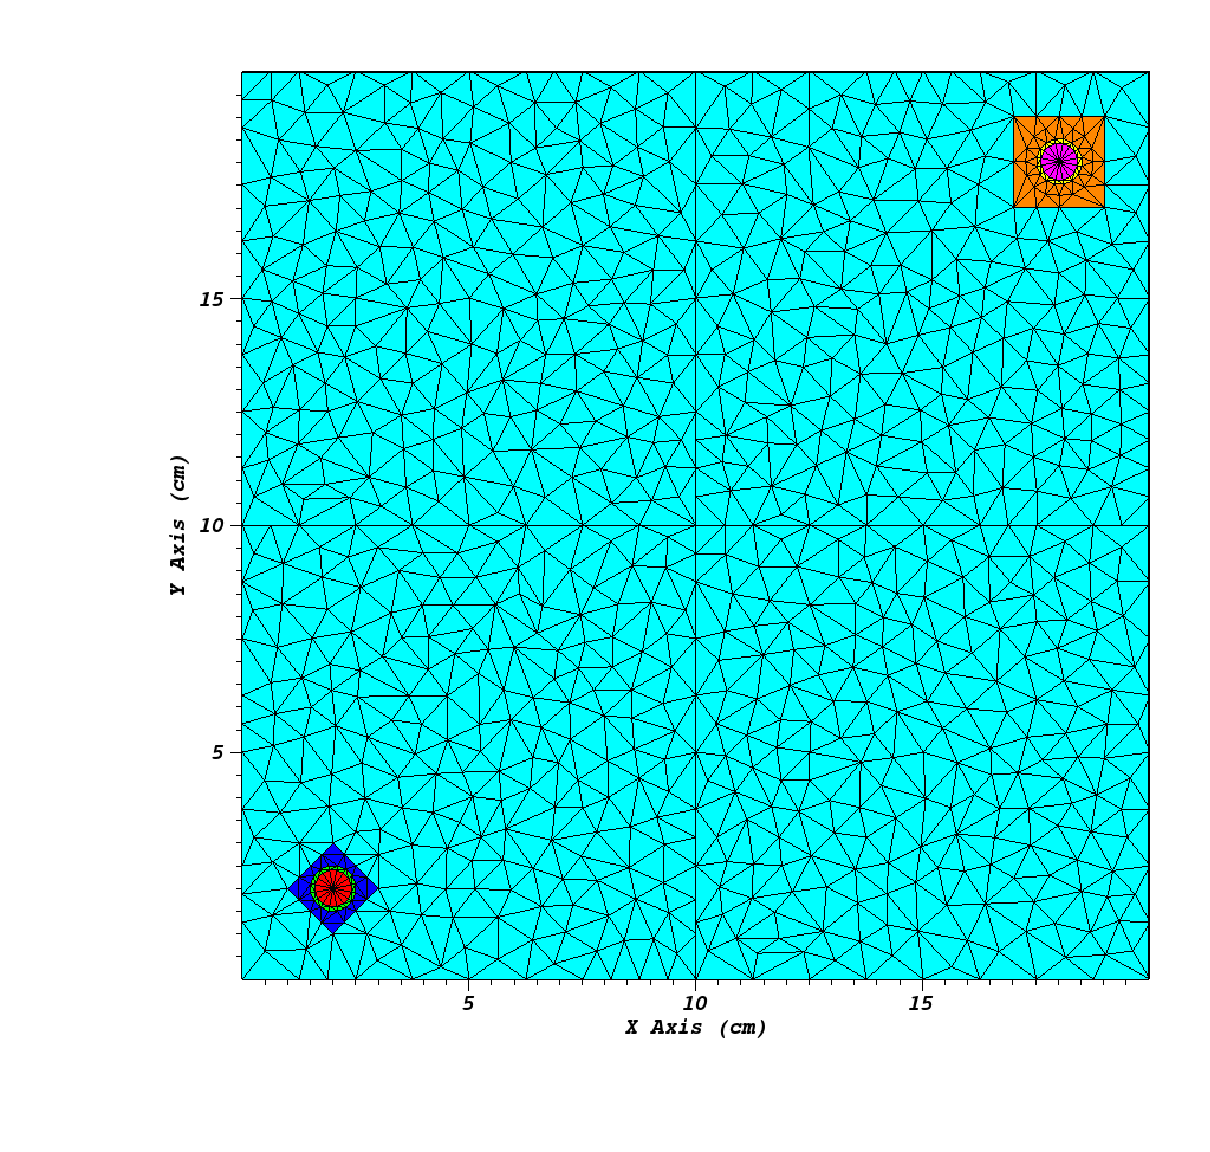
\includegraphics[scale=0.45,trim={0.95in 0.64in 0.35in 0.44in},clip]{figures/partitioning_example.pdf}
\end{frame}

\begin{frame}[t]\frametitle{Cubit vs. Triangle Meshes}
\begin{columns}

\begin{column}{.49\textwidth}
\begin{block}{Triangle}
  \begin{itemize}
    \item PDT meshes on the fly and in parallel by calling Triangle library.
    \item Stitching of ``hanging nodes" required.
    \item 2D extruded mesh.
  \end{itemize}
\end{block}
\end{column}

\begin{column}{.49\textwidth}
\begin{block}{Cubit}
  \begin{itemize}
    \item Mesh is generated, load balanced and then read into PDT (collaborative code with Rick Vega).
    \item No stitching necessary.
    \item First instance of a truly unstructured 3D mesh in PDT.
    \item More control over the mesh.
  \end{itemize}
\end{block}
\end{column}
\end{columns}
\end{frame}

\begin{frame}[t]\frametitle{Comparison of the two meshing approaches}
\centering
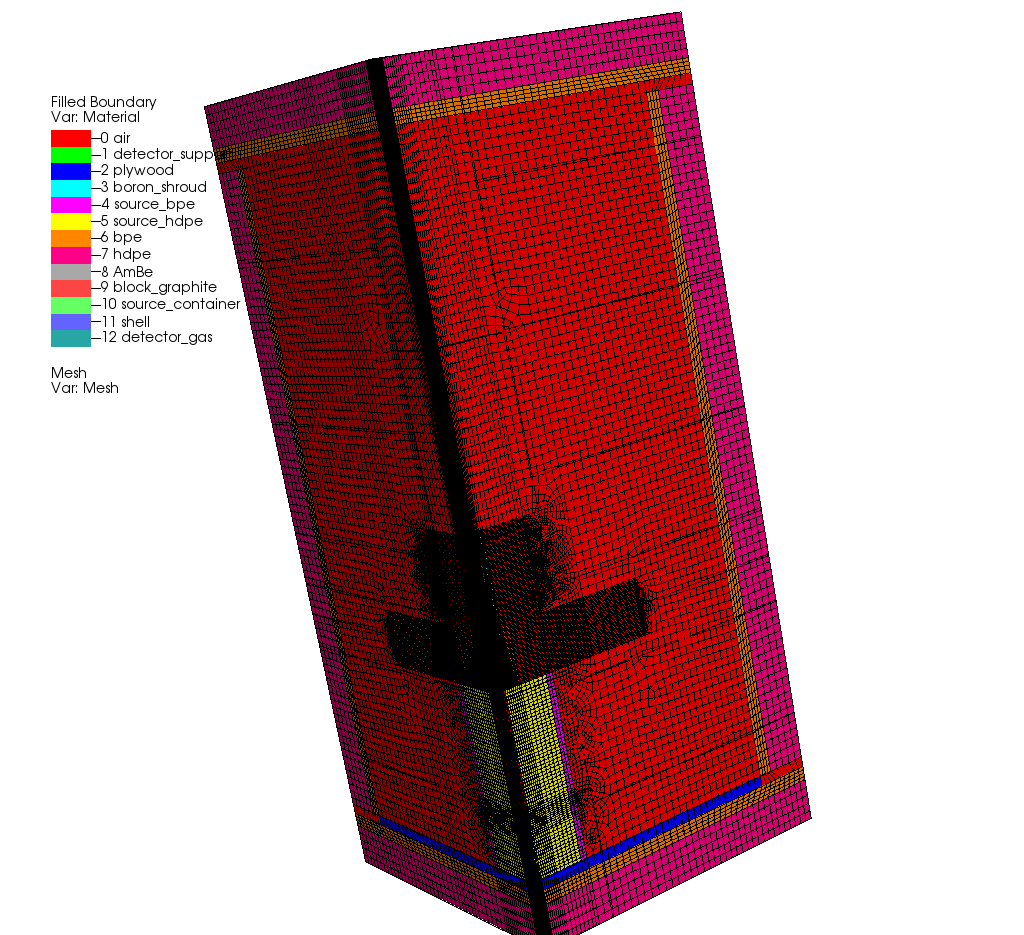
\includegraphics[scale=0.17]{../figures/im1_228.png}
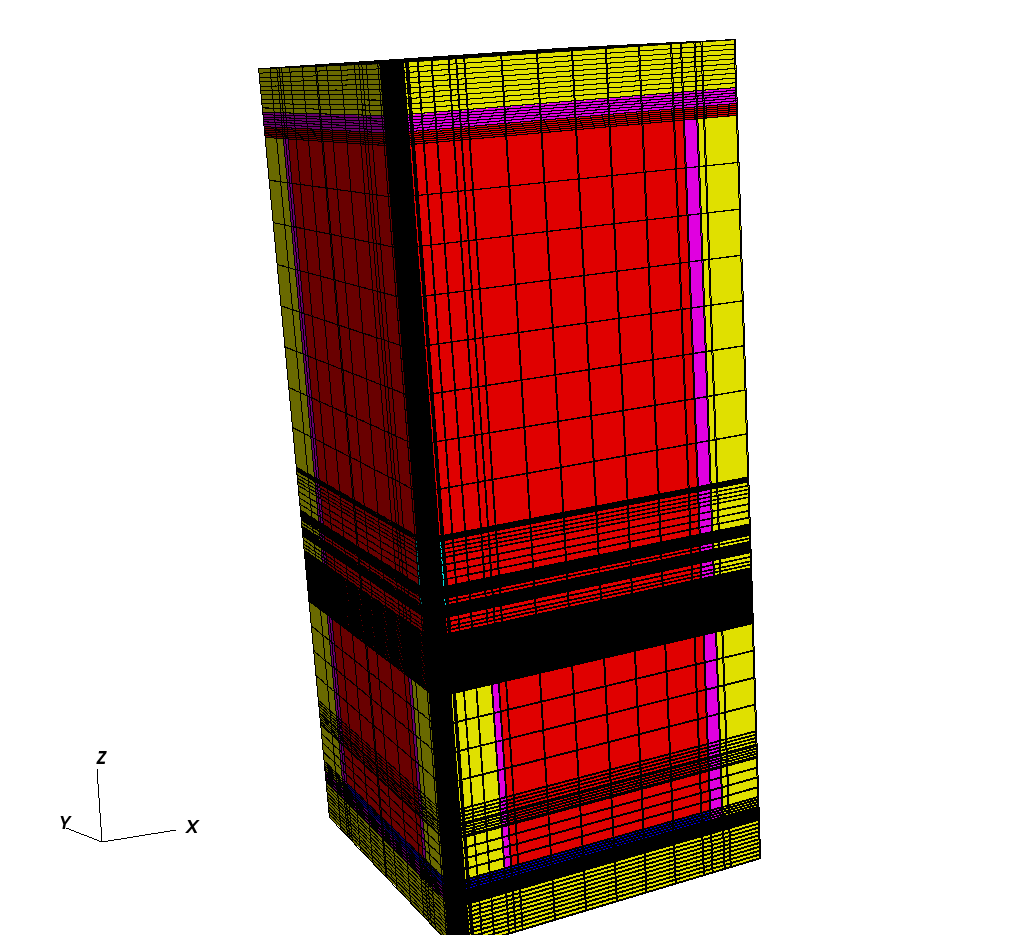
\includegraphics[scale=0.17]{../figures/im1c_prism.png}
\end{frame}

\section{Load Balancing Algorithms}

\begin{frame}[t]\frametitle{Load Balancing}
\begin{block}{Load Balance Metric}
  \begin{itemize}
    \item Max cells per subdomain divided by the average cells per subdomain:
      \begin{itemize}
        \item$f =\frac{\underset{ij}{\text{max}}(N_{ij})}{\frac{N_{tot}}{I\cdot J}}$
      \end{itemize}
    \item Column-wise metric: $f_I = \underset{i}{\text{max}}[\sum_{j} N_{ij}]/\frac{N_{tot}}{I}$
    \item Row-wise metric: $f_J = \underset{j}{\text{max}}[\sum_{i} N_{ij}]/\frac{N_{tot}}{J}$
    \item Per Column row-wise metric: $f_{J_i} = \text{max}[N_{ij}]_i/\frac{\sum_{j}N_{ij}}{J_i}$
  \end{itemize}		
  \tcr{Goal: minimize $f$ using locations of cut lines in X and Y}\\
    
  Subsequent improvement in algorithm: once dimension 1 has been balanced, balance dimension 2, then balance dimension 3 (\tcr{load balancing by dimension})
\end{block}
\end{frame}
\begin{frame}[t]\frametitle{Load Balancing Metrics}
\begin{equation}
f =\frac{\underset{ijk}{\text{max}}(N_{ijk})}{\frac{N_{tot}}{I\cdot J\cdot K}},
\label{metric_def}
\end{equation}
\begin{align}
f_{D1} &= \underset{d1}{\text{max}}[\sum_{d2,d3} N_{ijk}]/\frac{N_{tot}}{D1}, \label{f_d1} \\
f_{D2,d1} &= \Big(\underset{d2}{\text{max}}[\sum_{d3} N_{ijk,d1}]/\frac{N_{d1}}{D2}\Big), \label{f_d2}\\
f_{D3,d2,d1} &= \Big( \underset{d3}{\text{max}}[ N_{ijk,d1,d2}]/\frac{N_{d1,d2}}{D3} \Big) . \label{f_d3}
\end{align}
\end{frame}

\begin{frame}[t]\frametitle{Original Load Balancing Algorithm}
\begin{algorithm}[H]
\label{initial_algorithm}
\begin{algorithmic}

\WHILE{$f > \text{tol}_{\text{subset}}$}
  \IF {$f_I > \text{tol}_{\text{col}}$}
    \STATE Redistribute the X cut planes.
  \ENDIF
  \IF {$f_J > \text{tol}_{\text{row}}$}
  	\STATE Redistribute the Y cut planes.
  \ENDIF
\ENDWHILE
\end{algorithmic}
\end{algorithm}
\end{frame}

\begin{frame}[t]\frametitle{Theoretical Motivation for LBD}
  \begin{block}{}
  \begin{itemize}
    \item Consider simple 2D layout with $M$ unaligned patches of high mesh density
    \item The cellset layout is $[M(N+1)+1] \times [M(N+1)+1]$ but only $MN^2$ cellsets have much work.
    \item Load Imbalance Factor $= \frac{\left( M(N+1)+1 \right)^2}{MN^2} \xrightarrow{N\to \infty} \frac{M^2N^2}{MN^2} = M$
  \end{itemize}
  \end{block}
  \begin{center}
    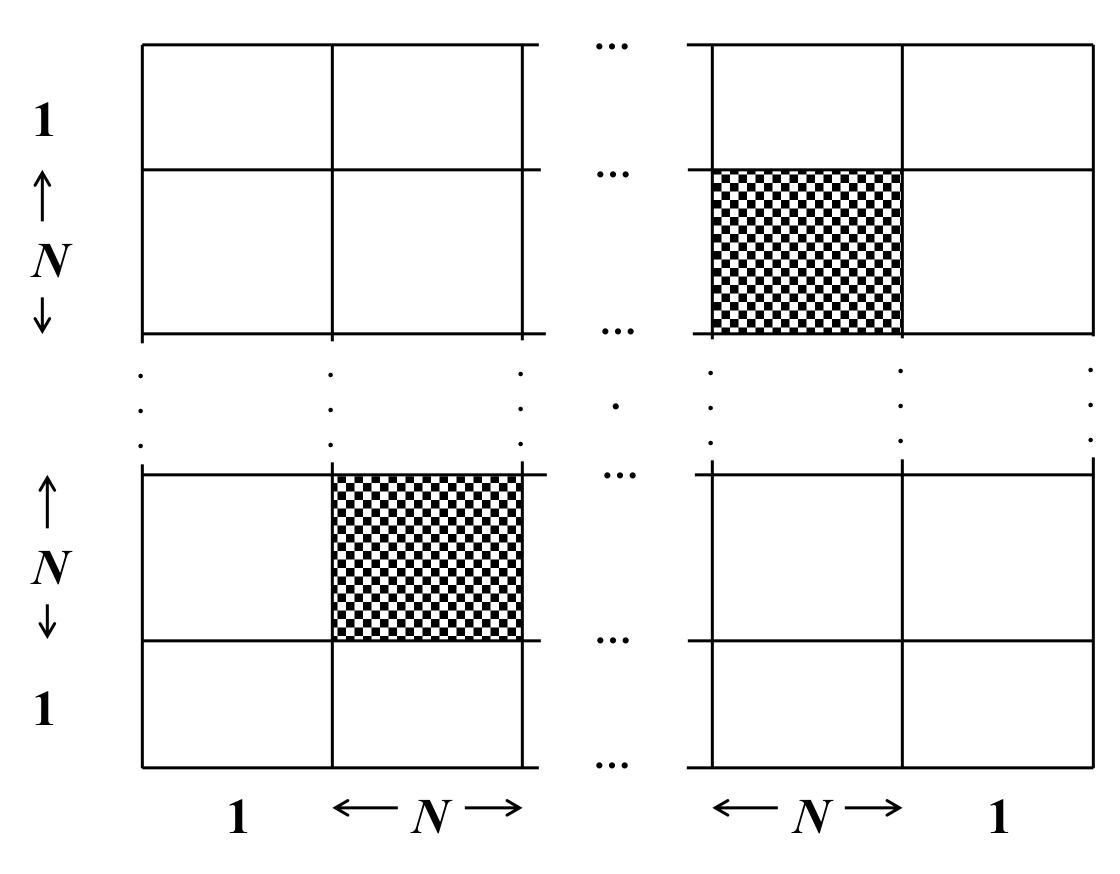
\includegraphics[width=5cm ]{figures/2dgeneral.png}
  \end{center}
\end{frame}

\begin{frame}[t]\frametitle{Load Balancing By Dimension Algorithm}
\begin{algorithm}[H]
\label{lbd}
\begin{algorithmic}

  \WHILE {$f_{D1} > \text{tol}_{\text{D1}}$}
    \STATE Redistribute the D1 cut planes.
  \ENDWHILE  
  
  \FOR {$d1$ in $D1$}
    \WHILE {$f_{D2,d1} > \text{tol}_{\text{D2}}$}
      \STATE Redistribute the D2 cut planes within d1. 
    \ENDWHILE
  \ENDFOR
  
  \FOR{$d1$ in $D1$}
    \FOR{$d2$ in $D2$}
      \WHILE {$f_{D3,d2,d1} > \text{tol}_{\text{D3}}$ }
        \STATE Redistribute the D3 cut planes within d2 within d1. 
      \ENDWHILE
    \ENDFOR
  \ENDFOR
  
  \STATE Calculate $f$.
\end{algorithmic}
\end{algorithm}
\end{frame}

\begin{frame}[t]\frametitle{Redistribution}
\begin{figure}[H]
\centering
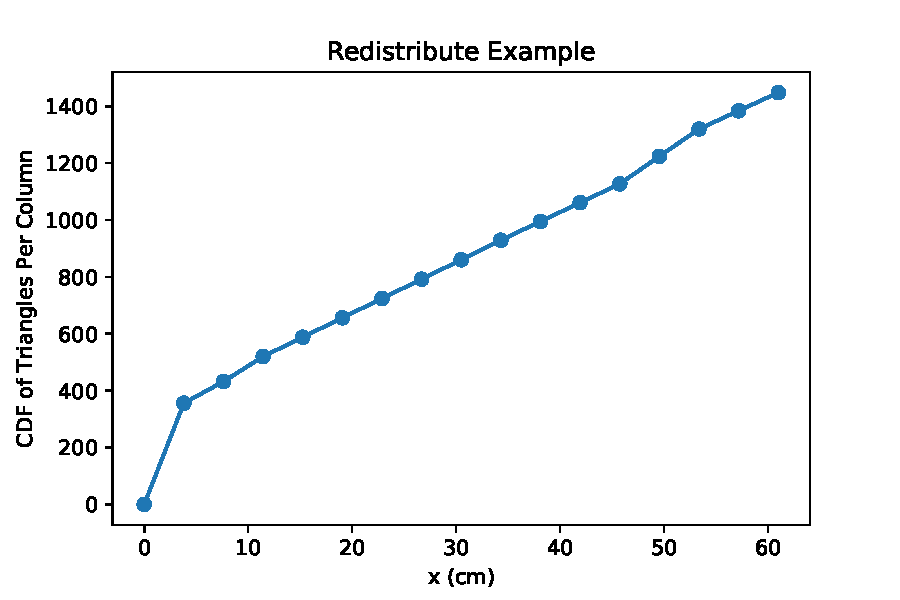
\includegraphics[scale=0.3]{figures/redistribute_before.pdf}
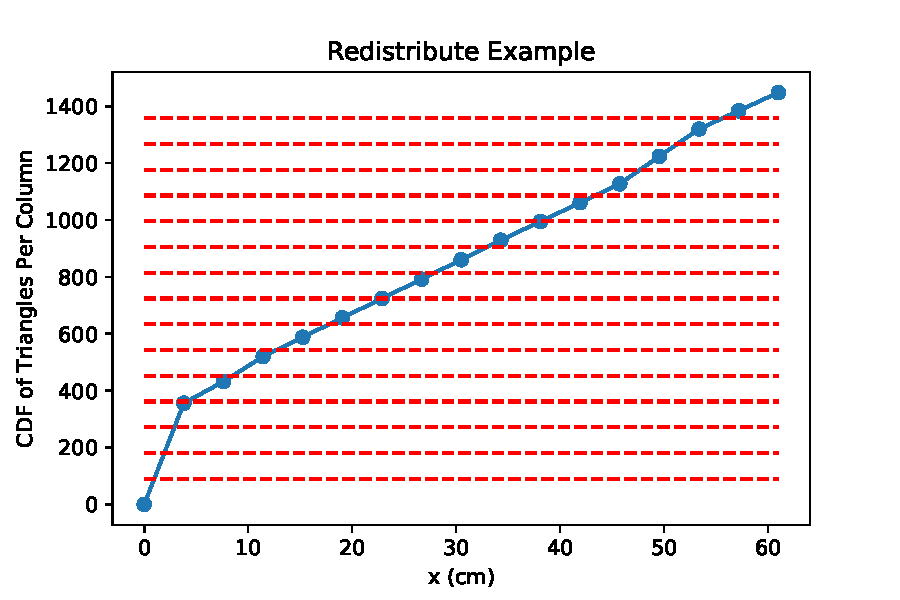
\includegraphics[scale=0.3]{figures/redistribute_after.pdf}
\caption{The use of the CDF of triangles per column to redistribute the cut planes in X.}
\label{redistribute}
\end{figure}
\end{frame}


\begin{frame}[t]\frametitle{No Load Balancing, f = 41.82}
\centering
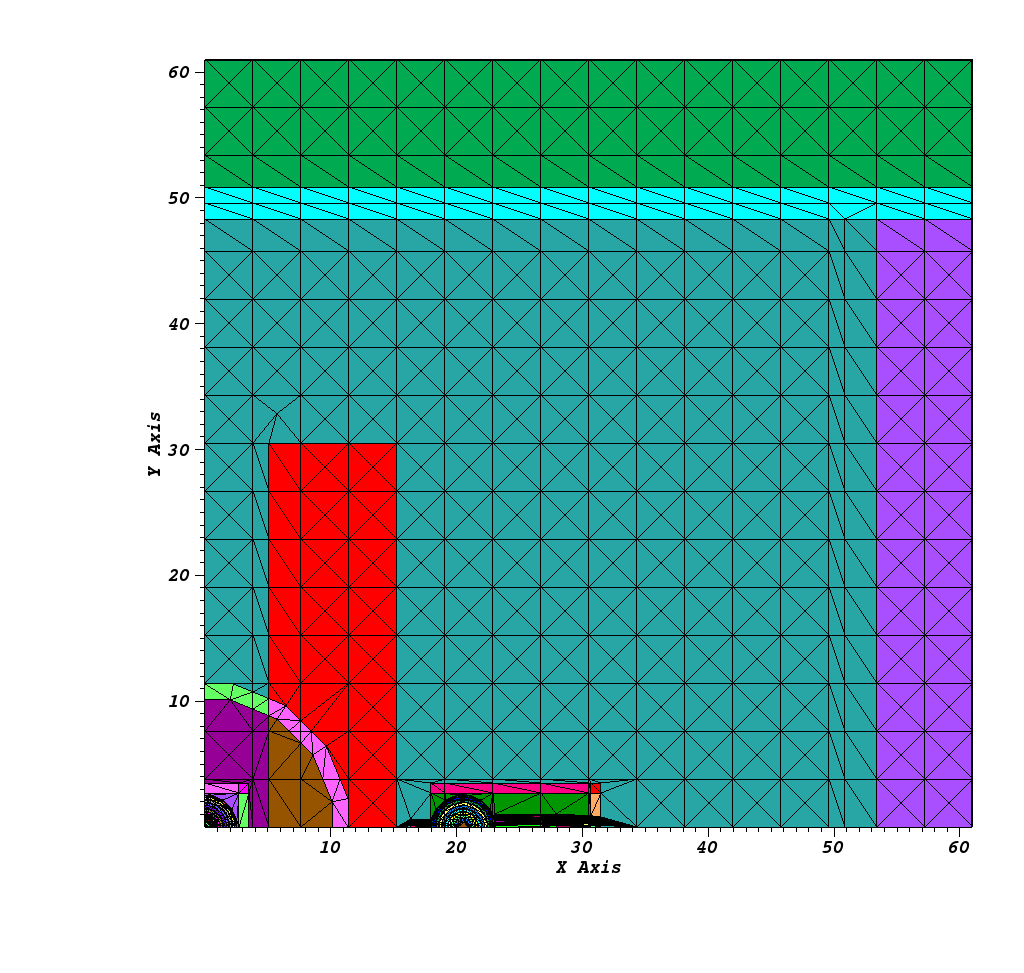
\includegraphics[scale=0.25]{figures/im12d_nolb.png}
\end{frame}

\begin{frame}[t]\frametitle{Load Balancing, f = 2.97}
\centering
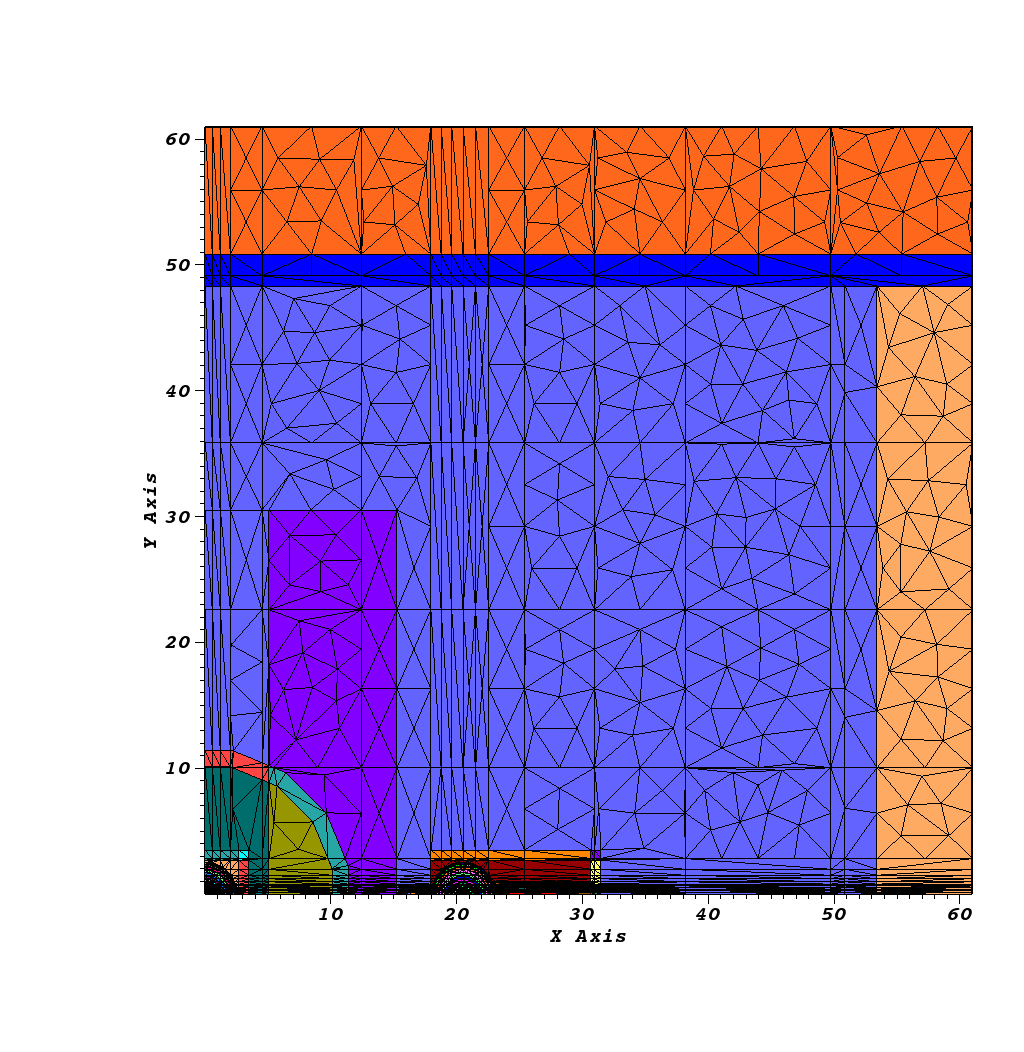
\includegraphics[trim={1cm 0cm 0cm 3cm},clip,scale=0.25]{figures/im12d_oldlb.png}
\end{frame}


\begin{frame}[t]\frametitle{Load Balancing By Dimension, f = 2.02}
\centering
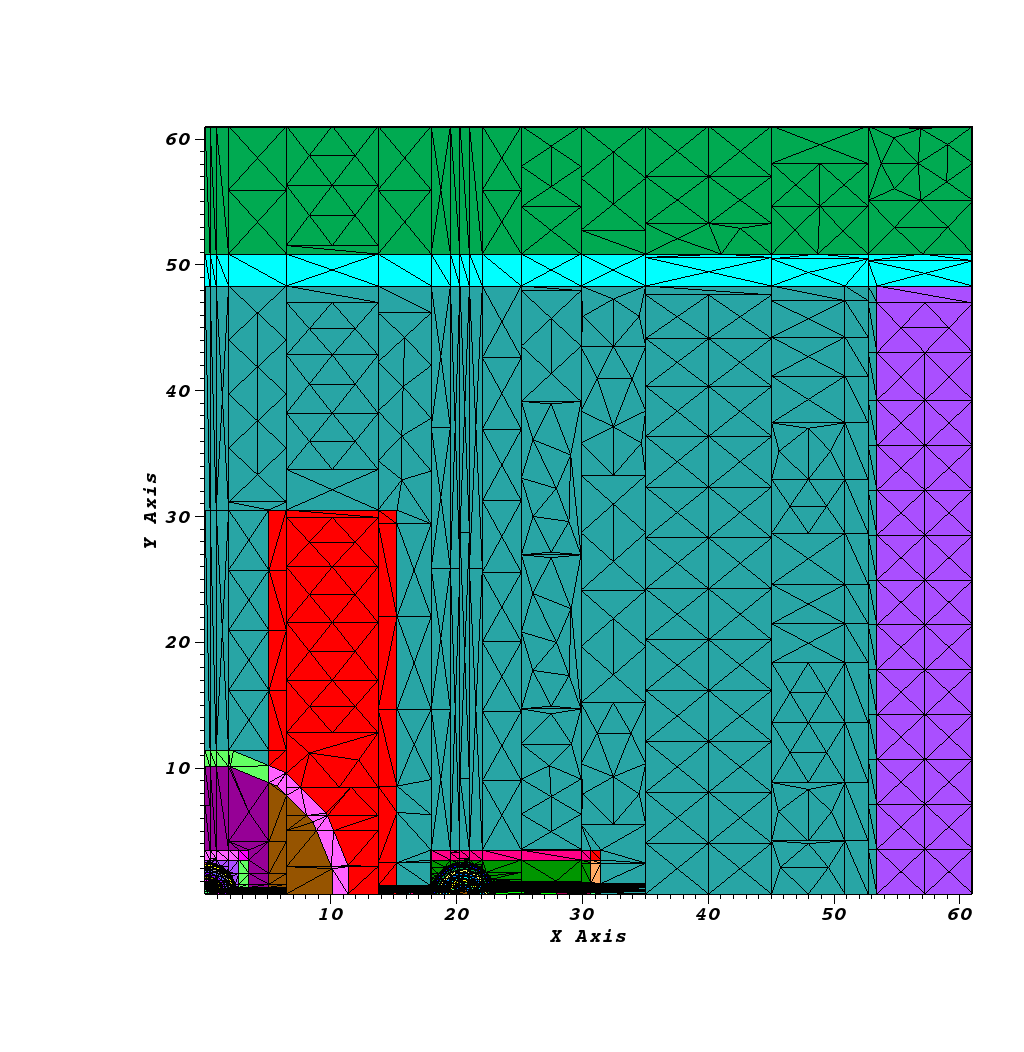
\includegraphics[scale=0.22]{figures/im12d_newlb.png}
\end{frame}

\begin{frame}[t]\frametitle{3D Load Balancing By Dimension}
\centering
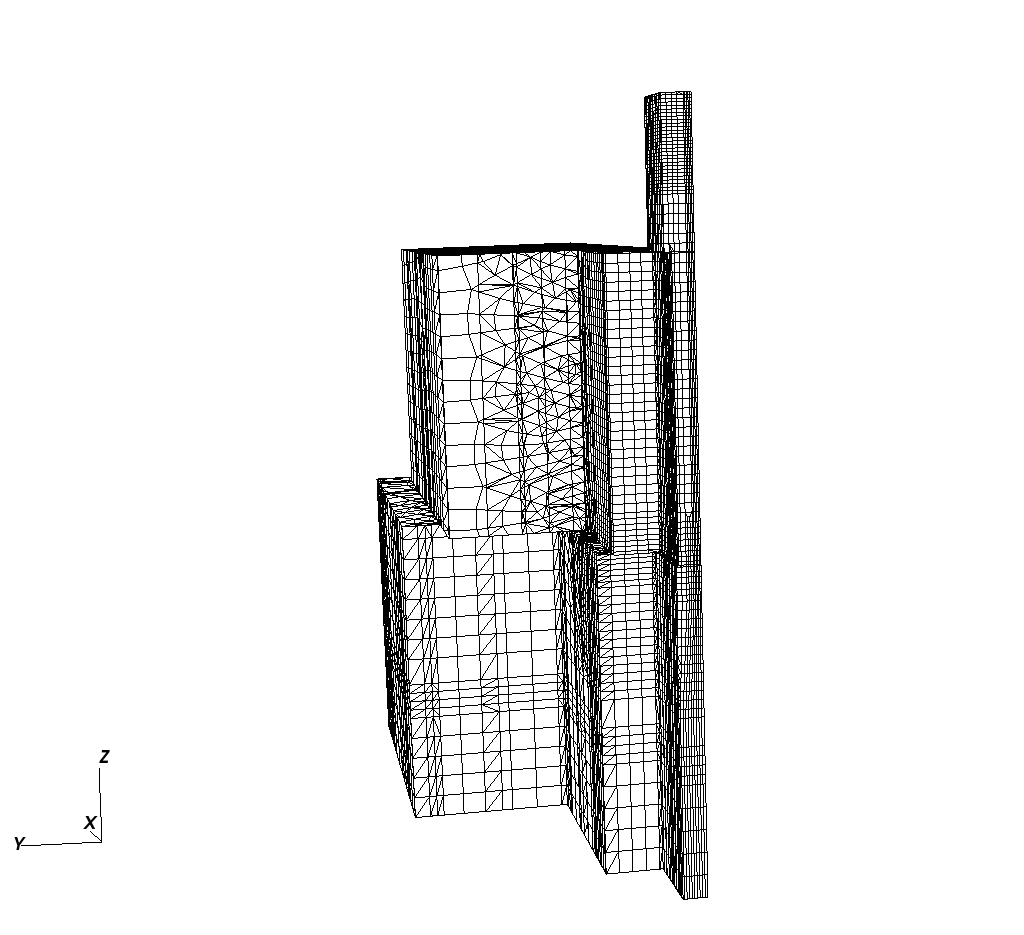
\includegraphics[trim={0cm 1cm 0cm 3cm},clip,scale=0.27]{figures/im1_foam_448.png}
\end{frame}

\begin{frame}[t]\frametitle{Load Balancing Study}
\begin{figure}[H]
\centering
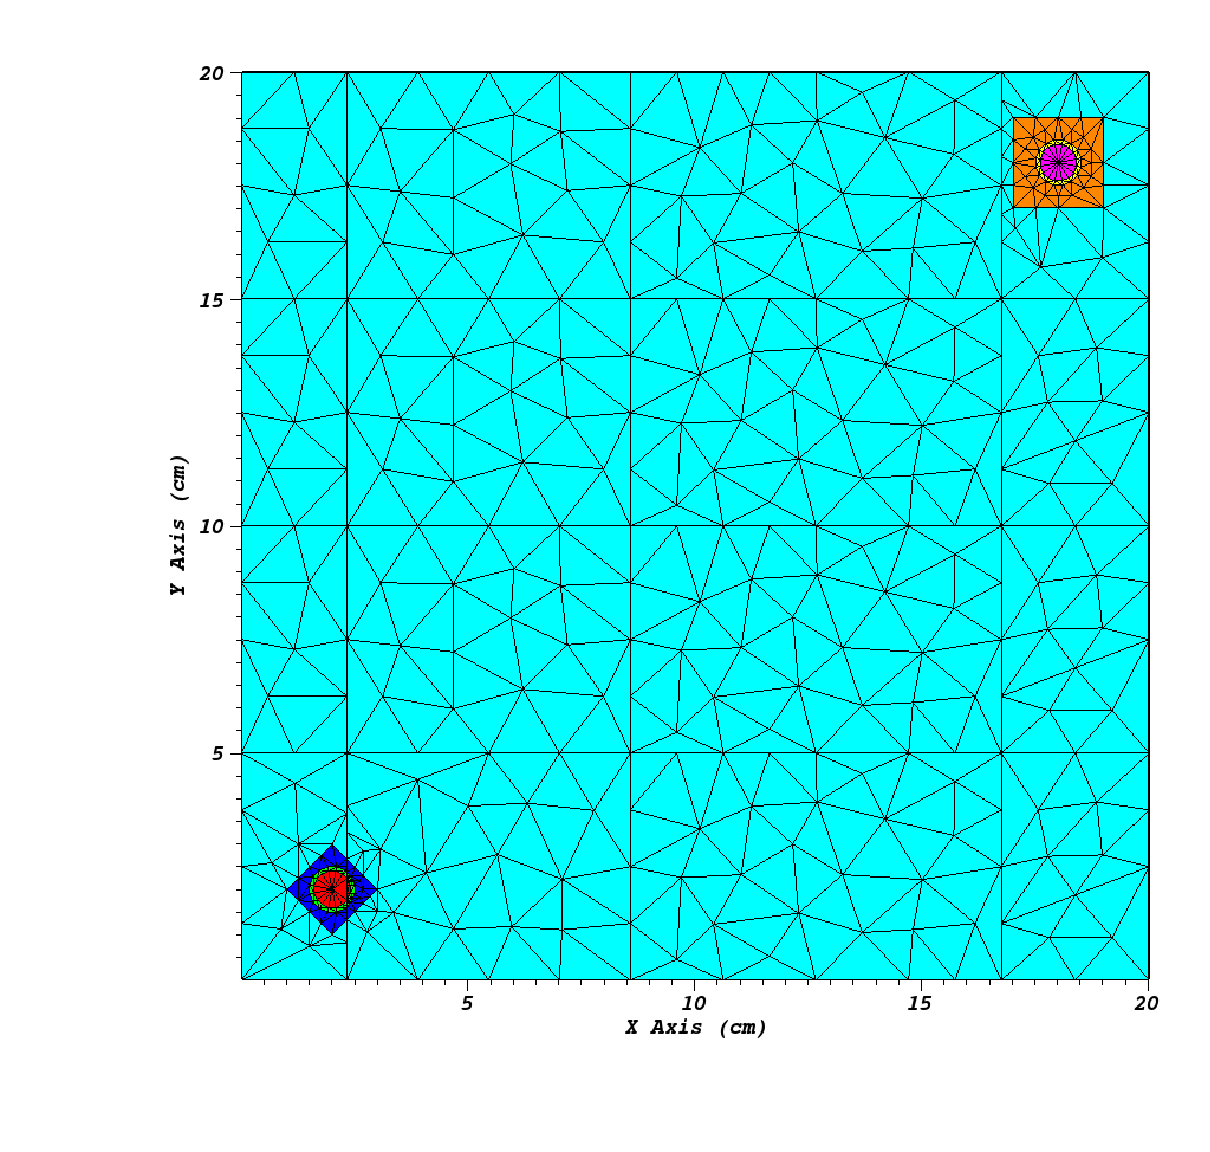
\includegraphics[scale=0.25,trim={0.95in 0.64in 0.35in 0.44in},clip]{figures/og_lb_example.pdf}
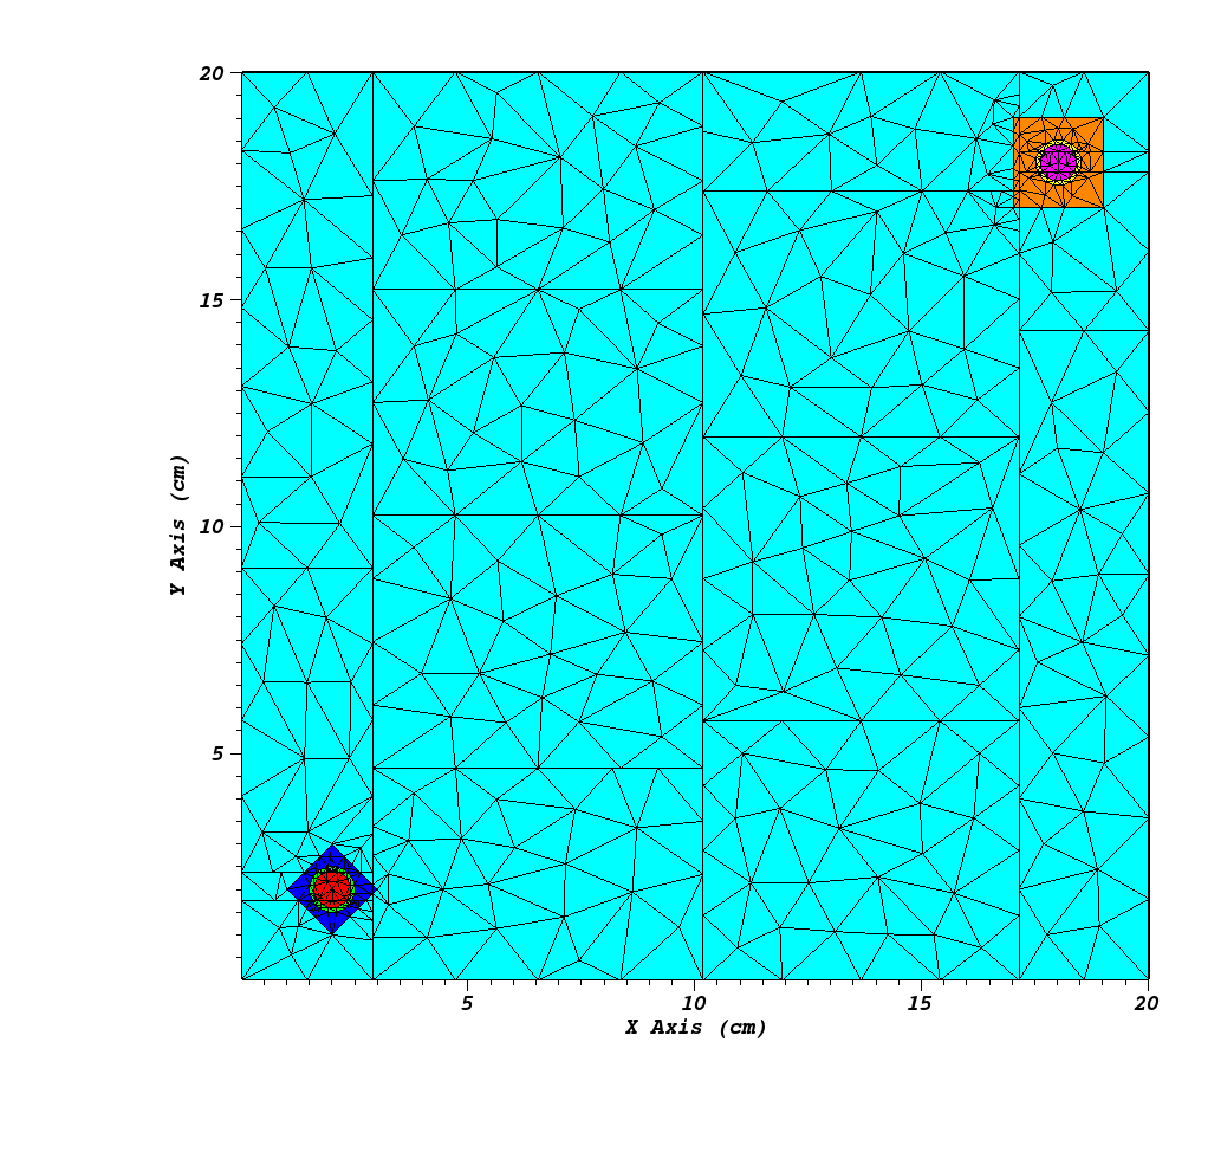
\includegraphics[scale=0.25,trim={0.95in 0.64in 0.35in 0.44in},clip]{figures/lbd_example.pdf}
\label{alg_illustration}
\end{figure}
  \begin{block}{Parametric Study Parameters}
    \begin{itemize}
      \item Number of subsets ranging from 2 to 10 each in $x$ and $y$.
      \item Maximum triangle area ranging from coarsest possible to 0.01 cm\textsuperscript{2}.
      \item Minimum triangle angle kept constant at $20^{\circ}$.
    \end{itemize}
  \end{block}
\end{frame}

\begin{frame}[t]\frametitle{Load Balancing Study}
\begin{table}[H]
\centering
\caption{\bf The percent improvement of the original load balancing algorithm (left) and the load balancing by dimension algorithm (right).}
\scalebox{0.4}{
\begin{tabular}{c|c|c|c|c|c|c|c|c|c} 

\bf Area, $N^{1/2}$ & \bf  2 & \bf 3    &  \bf  4   &  \bf  5   &  \bf 6    &  \bf  7   &   \bf 8   &  \bf 9    &  \bf 10   \\ \hline \hline
\bf Coarse& 0.000 & 0.367 & 0.403 & 0.552 & 0.628 & 0.491 & 0.890 & 0.720 & 0.765 \\ \hline 
 \bf 1.8& 0.000 & 0.091 & 0.337 & 0.364 & 0.473 & 0.390 & 0.767 & 0.413 & 0.683 \\ \hline 
 \bf 1.6& 0.000 & 0.093 & 0.398 & 0.368 & 0.499 & 0.370 & 0.815 & 0.353 & 0.774 \\ \hline 
 \bf 1.4& 0.000 & 0.061 & 0.080 & 0.410 & 0.415 & 0.412 & 0.570 & 0.413 & 0.545 \\ \hline 
 \bf 1.2& 0.000 & 0.007 & 0.391 & 0.340 & 0.378 & 0.315 & 0.536 & 0.245 & 0.196 \\ \hline 
 \bf 1.0& 0.000 & 0.038 & 0.206 & 0.420 & 0.341 & 0.186 & 0.696 & 0.201 & 0.160 \\ \hline 
 \bf 0.8& 0.000 & 0.049 & 0.109 & 0.336 & 0.434 & 0.139 & 0.637 & 0.228 & 0.000 \\ \hline 
 \bf 0.6& 0.000 & 0.000 & 0.057 & 0.199 & 0.163 & 0.346 & 0.517 & 0.000 & 0.090 \\ \hline 
 \bf 0.4& 0.000 & 0.000 & 0.065 & 0.013 & 0.267 & 0.147 & 0.528 & 0.179 & 0.000 \\ \hline 
 \bf 0.2& 0.000 & 0.000 & 0.000 & 0.000 & 0.001 & 0.041 & 0.566 & 0.121 & 0.000 \\ \hline 
 \bf 0.1& 0.000 & 0.000 & 0.000 & 0.000 & 0.000 & 0.000 & 0.540 & 0.089 & 0.000 \\ \hline 
 \bf 0.08&0.000 & 0.000 & 0.000 & 0.000 & 0.000 & 0.000 & 0.458 & 0.000 & 0.000 \\ \hline 
 \bf 0.06&0.000 & 0.000 & 0.000 & 0.000 & 0.000 & 0.000 & 0.409 & 0.000 & 0.000 \\ \hline 
 \bf 0.05&0.000 & 0.000 & 0.000 & 0.000 & 0.000 & 0.000 & 0.360 & 0.000 & 0.000 \\ \hline 
 \bf 0.04&0.000 & 0.000 & 0.000 & 0.000 & 0.000 & 0.000 & 0.348 & 0.000 & 0.000 \\ \hline 
 \bf 0.03&0.000 & 0.000 & 0.000 & 0.000 & 0.000 & 0.000 & 0.293 & 0.000 & 0.000 \\ \hline 
 \bf 0.02&0.000 & 0.000 & 0.000 & 0.000 & 0.000 & 0.000 & 0.000 & 0.000 & 0.000 \\ \hline 
 \bf 0.01&0.000 & 0.000 & 0.000 & 0.000 & 0.000 & 0.000 & 0.000 & 0.000 & 0.000 \\ \hline 
\end{tabular}}
\scalebox{0.4}{
\begin{tabular}{c|c|c|c|c|c|c|c|c|c} 
\bf Area, $N^{1/2}$ & \bf  2 & \bf 3    &  \bf  4   &  \bf  5   &  \bf 6    &  \bf  7   &   \bf 8   &  \bf 9    &  \bf 10   \\ \hline \hline
\bf Coarse& 0.175 & 0.663 & 0.743 & 0.781 & 0.796 & 0.757 & 0.938 & 0.760 & 0.820 \\ \hline 
  \bf 1.8& 0.266 & 0.417 & 0.511 & 0.661 & 0.766 & 0.665 & 0.896 & 0.647 & 0.512 \\ \hline 
  \bf 1.6& 0.262 & 0.426 & 0.568 & 0.635 & 0.760 & 0.631 & 0.897 & 0.542 & 0.557 \\ \hline 
  \bf 1.4& 0.244 & 0.369 & 0.497 & 0.618 & 0.769 & 0.595 & 0.901 & 0.722 & 0.741 \\ \hline 
  \bf 1.2& 0.242 & 0.336 & 0.552 & 0.614 & 0.663 & 0.583 & 0.886 & 0.208 & 0.597 \\ \hline 
  \bf 1.0& 0.203 & 0.287 & 0.458 & 0.549 & 0.442 & 0.605 & 0.875 & 0.536 & 0.552 \\ \hline 
  \bf 0.8& 0.162 & 0.330 & 0.435 & 0.460 & 0.638 & 0.542 & 0.888 & 0.393 & 0.000 \\ \hline 
  \bf 0.6& 0.122 & 0.291 & 0.447 & 0.460 & 0.503 & 0.610 & 0.844 & 0.267 & 0.058 \\ \hline 
  \bf 0.4& 0.093 & 0.274 & 0.310 & 0.400 & 0.488 & 0.519 & 0.888 & 0.328 & 0.000 \\ \hline 
  \bf 0.2& 0.042 & 0.147 & 0.185 & 0.267 & 0.344 & 0.299 & 0.810 & 0.349 & 0.025 \\ \hline 
  \bf 0.1& 0.026 & 0.067 & 0.109 & 0.156 & 0.144 & 0.210 & 0.735 & 0.367 & 0.000 \\ \hline 
  \bf 0.08&0.002 & 0.032 & 0.059 & 0.060 & 0.122 & 0.150 & 0.699 & 0.268 & 0.041 \\ \hline 
  \bf 0.06&0.005 & 0.014 & 0.036 & 0.057 & 0.094 & 0.073 & 0.643 & 0.246 & 0.058 \\ \hline 
  \bf 0.05&0.006 & 0.017 & 0.006 & 0.005 & 0.033 & 0.068 & 0.579 & 0.208 & 0.008 \\ \hline 
  \bf 0.04&0.002 & 0.008 & 0.009 & 0.000 & 0.011 & 0.022 & 0.544 & 0.168 & 0.000 \\ \hline 
  \bf 0.03&0.002 & 0.000 & 0.005 & 0.024 & 0.028 & 0.027 & 0.479 & 0.089 & 0.000 \\ \hline 
  \bf 0.02&0.003 & 0.002 & 0.001 & 0.000 & 0.001 & 0.004 & 0.361 & 0.070 & 0.000 \\ \hline 
  \bf 0.01&0.002 & 0.003 & 0.002 & 0.000 & 0.001 & 0.000 & 0.196 & 0.027 & 0.000 \\ \hline 

\end{tabular}}
\label{all_improvements}
\end{table}
\end{frame}

\begin{frame}[t]\frametitle{Paramtric Study Conclusions}
  \begin{block}{}
  \begin{itemize}
    \item The more uniformly refined your mesh, the more inherently balanced it is.
    \item With the exception of a few outliers, the load balancing by dimension algorithm was an improvement over the original load balancing algorithm.
    \item The metric improved by a max of 76.9\% and a mean of 21.7\% with the load balancing by dimension algorithm over the original load balancing algorithm. 
  \end{itemize}
  \end{block}
\end{frame}

\begin{frame}[t]\frametitle{Consequences of Load Balancing By Dimension}
  \begin{block}{}
  \begin{itemize}
    \item Perfect load balance in some cases will come at the cost of optimal sweeping.
    \item Time to solution is the most important parameter, and if keeping a more optimal sweeping grid means a less balanced problem, then so be it.
    \item The concept of a stage may be misleading when dealing with imbalanced partitions, as we cannot easily characterize the idle time.
    \item A time-to-solution estimator must be built to more accurately predict sweep time.
  \end{itemize}
  \end{block}
\end{frame}

\begin{frame}[t]\frametitle{Sweep on Regular Grid with 3 Angle Sets}
	\animategraphics[loop,controls,width=0.8\linewidth]{10}{figures/sweep_figs/sweeps_png/sweep_regular_20x20_as3_dog/sweep_regular_20x20_as3_dog_}{1}{48}
	%\href{run:figures/sweep_figs/sweeps_png/sweep_regular_20x20_as3_dog/animation.gif}{Animation.gif}
\end{frame}

\begin{frame}[t]\frametitle{Sweep on LBD Grid with 3 Angle Sets}
	\animategraphics[loop,controls,width=0.8\linewidth]{10}{figures/sweep_figs/sweeps_png/sweep_random_20x20_as3_dog/sweep_random_20x20_as3_dog_}{1}{101}
	%\href{run:figures/sweep_figs/sweeps_png/sweep_random_20x20_as3_dog/animation.gif}{Animation.gif}
\end{frame}


\begin{frame}[t]\frametitle{Sweep on Worst Grid with 1 Angle Set}
	\animategraphics[loop,controls,width=0.8\linewidth]{10}{figures/sweep_figs/sweeps_png/sweep_worst_20x20_as1_dog/sweep_worst_20x20_as1_dog_}{1}{230}
	%\href{run:figures/sweep_figs/sweeps_png/sweep_worst_20x20_as1_dog/animation.gif}{Animation.gif}
\end{frame}

\section{Partitioning Optimization on Unstructured Grids}

\begin{frame}[t]\frametitle{Overview}
\begin{block}{}
\begin{itemize}
	\item We need to optimize the cut line location not for balance, but for the best possible sweep time.
	\item We must build a time-to-solution estimator that calculates the time to solution for a given cut line partitioning.
	\item The time to solution estimator will be fed into an optimizing function that minimizes the time to solution. The cut lines corresponding to the minimum time to solution are the optimal partitioning scheme.
\end{itemize}
\end{block}
\end{frame}

\begin{frame}[t]\frametitle{Time to Solution Estimator}
\begin{block}{}
\begin{itemize}
  \item For a given partition, this tool will build subset-level (not cell level) directed task dependence graphs for each octant, and weight the edges of that graph based on a set of criteria.
  \item The estimator returns the maximum time to sweep across one of the graphs.
\end{itemize}
\end{block}
\begin{block}{}
\begin{equation}
\text{TOS} = f(P_x, P_y, P_z, \text{\textcolor{red}{cut lines, threads}, machine params})
\end{equation}
\end{block}
\begin{block}{Important Assumption}
This process assumes that there are NO cycles in the TDGs. All graphs are acyclic.
\end{block}
\end{frame}

\begin{frame}[t]\frametitle{Time to Solution Estimator}
\begin{block}{}
\begin{enumerate}
	\item Given a partitioning scheme (cut lines), build adjacency matrix.
	\item Build Directed Acyclic Graphs (DAGs) from the adjacency matrix, one for each octant.
	\item Weight the DAG's edges based on:
	\begin{itemize}
		\item Solve and communication time of each subset to its neighbors.
		\item Conflicts that arise between DAGs due to the sweep.
	\end{itemize}
	\item Compute solve time by getting the maximum final edge weight across all DAGs.
\end{enumerate}
\end{block}
\end{frame}

\begin{frame}[t]\frametitle{Weighting the Graphs}
\begin{block}{}
\begin{itemize}
	\item In order to weight the graph properly, we need to have a mesh density function that we can calculate the cells (and then unknowns) per subset from.
	\item The weight of the edge between two nodes (subsets) in the graph represents the solve and communication time of the base node.
\end{itemize}
\end{block}
\begin{block}{}
\begin{align}
\text{cells per subset} &= \int_{\tcr{x_i}}^{\tcr{x_{i+1}}} \int_{\tcr{y_j}}^{\tcr{y_{j+1}}} \int_{\tcr{z_k}}^{\tcr{z_{k+1}}} \text{mesh density } dx dy dz \\
\label{weight}
\text{weight} &= N_u\cdot T_u + N_b\cdot T_{\text{comm}} + \text{latency}\cdot M_L \\
N_u &= \text{num cells}\cdot \text{unknowns per cell} \\
N_b &\approx(\text{num boundary cells})\cdot \text{boundary unkowns per cell}
\end{align}
\end{block}
\end{frame}

\begin{frame}[t]\frametitle{Determining Cells per Subset}
	\centering
	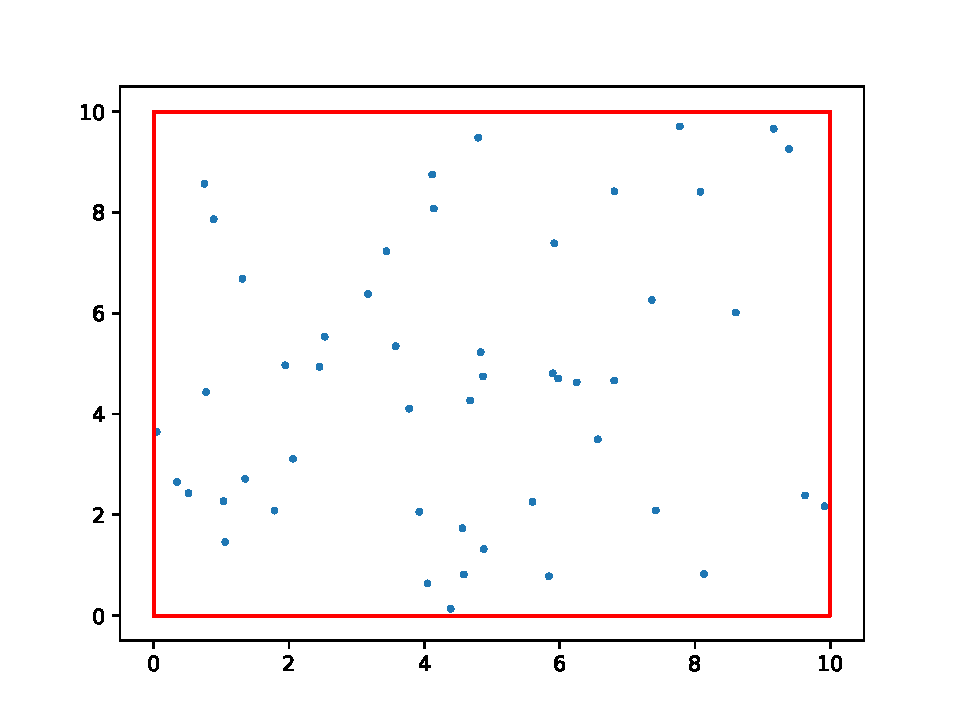
\includegraphics[scale=0.65]{figures/mesh_points.pdf}
\end{frame}

\begin{frame}[t]\frametitle{Determining Cells per Subset}
	\centering
	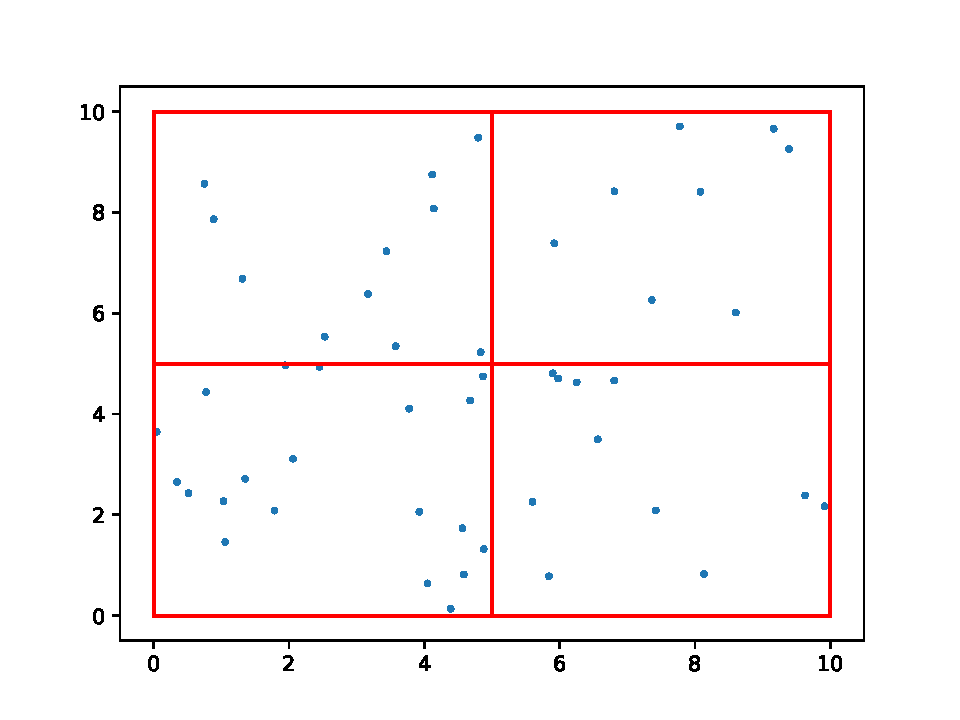
\includegraphics[scale=0.65]{figures/mesh_subsets.pdf}
\end{frame}

\begin{frame}[t]\frametitle{Universal Edge Weighting}
  \begin{block}{}
    \begin{itemize}
      \item Once the outgoing edges of each node are independently weighted, the next step is to have our graphs weighted on a universal time scale. 
      \item To do this, we calculate the sum of the longest weighted path to each node, and set all incoming edges to each node to this value.
      \item To find the longest weighted path, the graph weights are inverted, and the shortest weighted path is found. The original edge weights are used to calculate the value of the longest weighted path.
      \item The resulting graph is weighted so that the incoming edge to each node represents the time that node is ready to solve.
    \end{itemize}
  \end{block}
\end{frame}

\begin{frame}[t]\frametitle{Weighting Example}
  \centering
  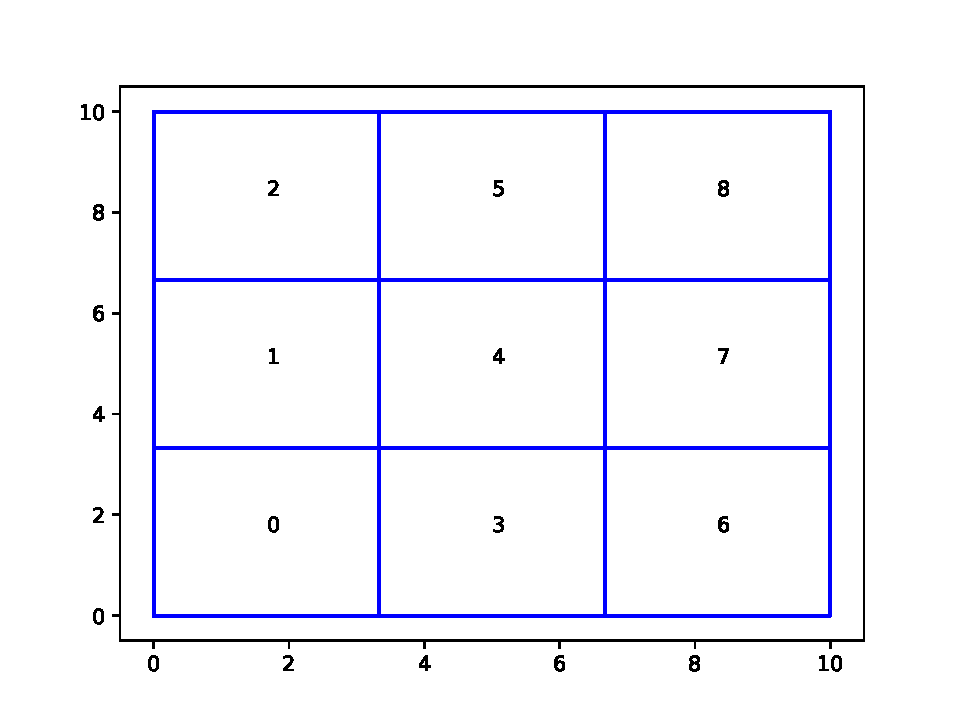
\includegraphics[scale=0.6]{figures/subset_plot_2d.pdf}
\end{frame}

\begin{frame}[t]\frametitle{Pre Universal Weighting}
  \centering
  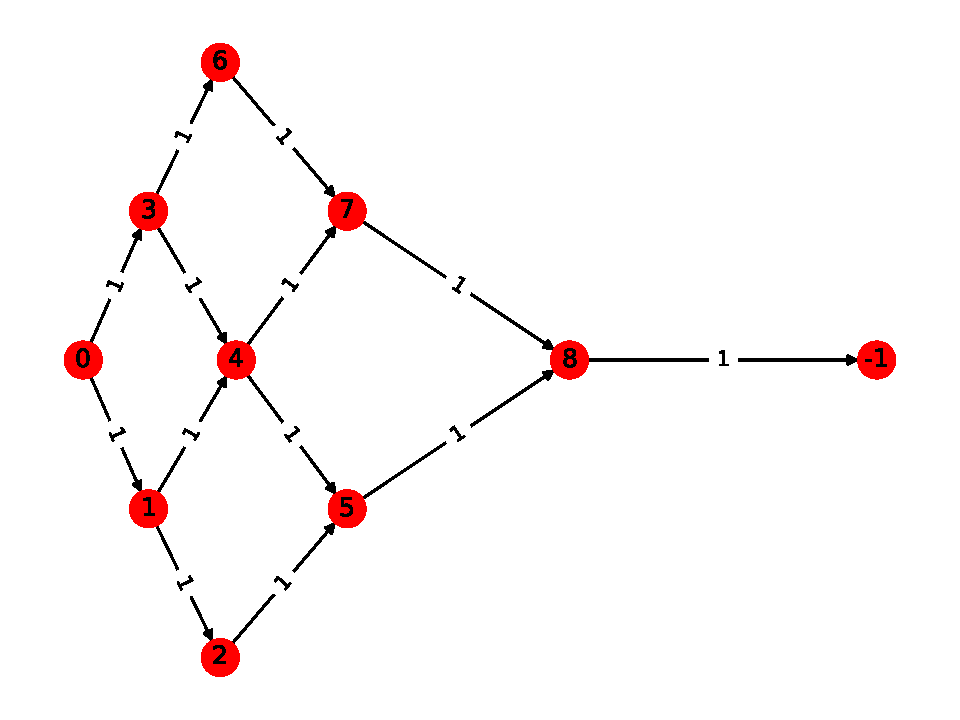
\includegraphics[scale=0.65]{figures/G_pre_universal.pdf}
\end{frame}

\begin{frame}[t]\frametitle{Post Universal Weighting}
  \centering
  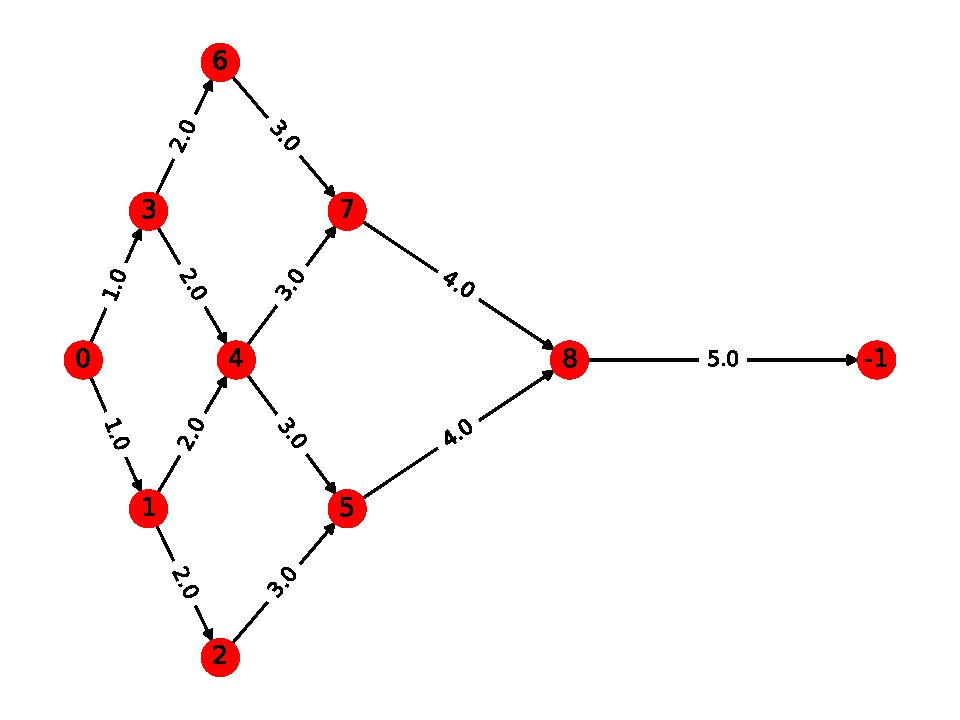
\includegraphics[scale=0.65]{figures/G_universal.pdf}
\end{frame}


\begin{frame}[t]\frametitle{Conflict Detection and Resolution}
\begin{block}{}
\begin{itemize}
	\item Once all edges in all TDGs are universaly weighted, we need to detect and resolve sweep conflicts between the 8 octants.
	\item For perfectly balanced and optimally partitioned problems (structured grids) we will default to a depth-of-graph conflict resolution (same as PDT).
	\item For unbalanced partitions, we will default to a first come first serve conflict resolution.
\end{itemize}
\end{block}
\end{frame}

\begin{frame}[t]\frametitle{First Come First Serve Conflict Resolution}
\begin{block}{}
\begin{itemize}
	\item The first octant to arrive to a node will begin solving it, and the remaining octants will incur a delay (if applicable).
	\item The delay is reflected in each remaining TDG by adding the corresponding delay as a weight to the applicable edge.
  \item If two octants arrive to a node at the same time, the octant with the greater remaining depth-of-graph and priority octant (same as PDT) wins the tie.
\end{itemize}
\end{block}
\begin{block}{Potential Future Work: hybrid depth-of-graph/first come first serve conflict resolution}
\begin{itemize}
	\item Two (or more) paths arrive to a node at different time, and when that node is free to solve, the path with the greater depth-of-graph remaining solves first.
\end{itemize}
\end{block}
\end{frame}

\begin{frame}[t]\frametitle{Conflict Resolution Algorithm}
  \begin{block}{}
    \begin{itemize}
      \item Best summarized as a ``marching" process. 
      \item Starting at time $t=0$, find the first interaction (recalling that the incoming weight to a node reflects the time it is ready to solve).
      \item If at time $t$, multiple TDGs are solving the same node, this means there is a conflict. 
      \item  ``Losing" TDGs modify their downstream weights according to how long they are delayed.
    \end{itemize}
  \end{block}
\end{frame}

\begin{frame}[t]\frametitle{Sweeping the Graph}
\begin{block}{}
\begin{itemize}
	\item Now that all TDGs are weighted based on solve time, communication time, and delays, we can easily calculate the time it takes each octant to sweep across the graph. 
	\item The maximum final edge weight across all TDGs is the maximum sweep time.
\end{itemize}
\end{block}
\end{frame}

\begin{frame}[t]\frametitle{Ongoing and Future Work}
  \begin{block}{}
    \begin{itemize}
      \item The time to solution estimator has been verified for 2D cases, with ongoing efforts for 3D verification.
      \item Preliminary optimization efforts are promising using the SciPy optimize library.  
      \item Numerical studies using comparing load balanced partitions vs. optimized partitions in PDT ongoing.
      \item Adding in support for multiple angles per octant. 
      \item Adding in support for angular and subset aggregation.
    \end{itemize}
  \end{block}
\end{frame}

\end{document}
